\pdfoutput=1
% PDF build (references and table/figure numbers): run from this directory
%   pdflatex report
%   bibtex report
%   pdflatex report
%   pdflatex report
% Or: latexmk -pdf -bibtex report.tex

\documentclass[11pt]{article}

\usepackage[final]{ACL/acl}

\usepackage{times}
\usepackage{latexsym}
\usepackage[T1]{fontenc}
\usepackage[utf8]{inputenc}
\usepackage{microtype}
\usepackage{inconsolata}
\usepackage{graphicx}
\usepackage{amsmath}
\usepackage{amssymb}
\usepackage{booktabs}
\usepackage{multirow}
\usepackage{xcolor}
\usepackage{subcaption}

\graphicspath{{figures/}}

\title{Comparative Study of Collaborative Filtering Methods\\for Movie Recommendation on MovieLens Latest}

\author{
  Yuting Zhou \\
  yuting.zhou@scarletmail.rutgers.edu \\
  \\\And
  Yiwei Li \\
  yiwei.li@scarletmail.rutgers.edu \\
}

\begin{document}
\maketitle

\begin{abstract}
Recommender systems are central to modern online platforms, yet choosing the right collaborative filtering strategy for a given dataset remains an open practical question. We implement and compare four collaborative filtering methods for movie recommendation on the \textbf{MovieLens Latest} corpus: biased matrix factorization with SGD (PyTorch), a deep hybrid model with CNN title and genre encoders, truncated-SVD with Ridge/Lasso calibration, and alternating least squares.
All models are evaluated on rating prediction (MAE, RMSE) and top-10 recommendation under an identical per-user 80/20 holdout split.
The deep hybrid model achieves the strongest overall profile, while tuned MF-SGD becomes a close second and attains the lowest RMSE.
SVD-Ridge/Lasso remain competitive linear baselines, and ALS still underperforms mainly on top-10 ranking quality under our current explicit-feedback configuration.
We provide training-dynamics analysis, auxiliary feature-block ablation on a smaller subset, and latent-factor discussion, and we ship a full-stack web demo (\textit{StreamX}) that serves the retrained checkpoints.
\end{abstract}



\section{Introduction}

Recommendation systems have become indispensable components of online services---from e-commerce product suggestions to movie and music discovery platforms \cite{ricci2011introduction}.
Among the many families of recommendation algorithms, \emph{collaborative filtering} (CF) relies exclusively on observed user--item interactions to infer preferences, making it applicable even when item content metadata is scarce \cite{resnick1994grouplens}.
The most successful CF paradigm to date is \emph{matrix factorization} (MF), which projects users and items into a shared latent space so that inner products approximate observed ratings \cite{koren2009matrix}.

Despite its conceptual simplicity, the design space of MF-based recommenders is vast.
Optimization may proceed via stochastic gradient descent (SGD), alternating least squares (ALS), or singular value decomposition (SVD);
the loss function may be mean squared error, Huber loss, or a ranking-aware surrogate;
and the model may incorporate side information such as item titles, genres, or temporal signals \cite{zhang2019deep}.
How these choices interact in practice---especially on a moderately sized, long-tailed dataset---is rarely benchmarked in a controlled, apples-to-apples fashion within a single codebase.

In this project, we address that gap by implementing four distinct collaborative filtering models from scratch, training all of them on the identical MovieLens Latest split, and evaluating them with the same metrics suite.
Our contributions are threefold:
\begin{itemize}
\item We provide a controlled comparison of four CF models---MF-SGD, a deep hybrid CNN model, SVD with linear calibration (Ridge/Lasso), and ALS---under identical data conditions.
\item We analyze not only aggregate accuracy (MAE, RMSE) and ranking quality (Precision, Recall, F1, NDCG@10) but also training dynamics, latent factor semantics, and feature-block ablation.
\item We build \textit{StreamX}, an end-to-end web application (Django\,+\,Next.js) that serves real-time recommendations from the trained models, demonstrating practical deployment.
\end{itemize}



\section{Problem Definition}

We formalize the recommendation task as follows.
Let $\mathcal{U}$ and $\mathcal{I}$ denote the sets of users and items, respectively, and let $r_{ui}\in[0.5,5.0]$ be the rating that user $u$ assigns to item $i$.
The observed ratings form a sparse matrix $\mathbf{R}\in\mathbb{R}^{|\mathcal{U}|\times|\mathcal{I}|}$, where only a small fraction of entries are known (density $\approx$ 0.12\% on this corpus).

\paragraph{Rating Prediction.}
Given a training set $\mathcal{D}_\text{train}$ of observed $(u,i,r_{ui})$ triples, learn a function $\hat{r}:\mathcal{U}\times\mathcal{I}\to\mathbb{R}$ that minimizes the prediction error on held-out ratings $\mathcal{D}_\text{test}$.
Performance is measured by Mean Absolute Error (MAE) and Root Mean Squared Error (RMSE):
\begin{align}
\text{MAE} &= \frac{1}{|\mathcal{D}_\text{test}|}\sum_{(u,i)\in\mathcal{D}_\text{test}} |r_{ui}-\hat{r}_{ui}|, \\
\text{RMSE} &= \sqrt{\frac{1}{|\mathcal{D}_\text{test}|}\sum_{(u,i)\in\mathcal{D}_\text{test}} (r_{ui}-\hat{r}_{ui})^2}.
\end{align}

\paragraph{Top-$N$ Recommendation.}
For each user $u$, produce a ranked list of $N=10$ items that $u$ has not yet interacted with.
The quality of the list is measured against the held-out items in $\mathcal{D}_\text{test}$ via Precision@$N$, Recall@$N$, F1@$N$, and NDCG@$N$.
Items are ranked by descending predicted rating.


\section{Related Work}

\paragraph{Memory-Based CF.}
Early CF methods compute user--user or item--item similarities directly from the rating matrix and aggregate neighbor ratings for prediction \cite{resnick1994grouplens,sarwar2001item}.
While interpretable, these methods scale poorly and are sensitive to sparsity.

\paragraph{Matrix Factorization.}
Koren et al.\ \cite{koren2009matrix} demonstrated that biased matrix factorization, optimized via SGD, achieves state-of-the-art accuracy on the Netflix Prize dataset.
Hu et al.\ \cite{hu2008collaborative} proposed weighted ALS for implicit feedback, and Zhou et al.\ \cite{zhou2008large} developed large-scale parallel ALS.
Koren \cite{koren2008factorization} further extended MF with neighborhood integration and temporal dynamics.

\paragraph{Deep Recommenders.}
He et al.\ \cite{he2017neural} introduced Neural Collaborative Filtering, replacing the inner product with a multi-layer perceptron.
Cheng et al.\ \cite{cheng2016wide} proposed Wide\,\&\,Deep learning, combining memorization and generalization.
Covington et al.\ \cite{covington2016deep} described YouTube's two-tower deep recommendation architecture.
Wang et al.\ \cite{wang2015collaborative} combined deep autoencoders with CF.
More recently, Zhang et al.\ \cite{zhang2019deep} surveyed the landscape of deep-learning-based recommender systems.

\paragraph{Hybrid Approaches.}
Leveraging item content (titles, genres, descriptions) alongside collaborative signals has been shown to mitigate cold-start and improve generalization.
CNN-based text encoders, following Kim \cite{kim2014convolutional}, are commonly used to extract features from short textual metadata in recommendation contexts.

Our work brings together classical MF (SGD and ALS variants), an SVD-based linear hybrid, and a deep content-aware model within a single comparative framework.



\section{Methodology}

All four models share a common prediction structure:
\begin{equation}
\hat{r}_{ui} = \mu + b_u + b_i + \mathbf{p}_u^\top \mathbf{q}_i,
\label{eq:base}
\end{equation}
where $\mu$ is the global mean rating, $b_u$ and $b_i$ are user and item biases, and $\mathbf{p}_u,\mathbf{q}_i\in\mathbb{R}^k$ are latent factor vectors.
They differ in how the parameters are estimated and whether additional content features are incorporated.

\subsection{MF-SGD}

This model directly optimizes the $L_2$-regularized squared-error objective:
\begin{equation}
\min_{\mathbf{p},\mathbf{q},b} \sum_{(u,i)\in\mathcal{D}_\text{train}} \!\!\bigl(r_{ui} - \hat{r}_{ui}\bigr)^2 + \lambda\bigl(\|\mathbf{p}_u\|^2 + \|\mathbf{q}_i\|^2 + b_u^2 + b_i^2\bigr),
\label{eq:mfsgd}
\end{equation}
via element-wise SGD.
At each step, the error $e_{ui}=r_{ui}-\hat{r}_{ui}$ drives gradient updates:
$b_u \leftarrow b_u + \eta(e_{ui}-\lambda b_u)$,
$\mathbf{p}_u \leftarrow \mathbf{p}_u + \eta(e_{ui}\,\mathbf{q}_i - \lambda\,\mathbf{p}_u)$,
and symmetrically for $b_i$ and $\mathbf{q}_i$.

Key design choices on MovieLens Latest: latent dimension $k{=}128$, learning rate $\eta{=}0.0035$ with multiplicative decay $0.995{\times}$ per epoch, regularization $\lambda{=}0.04$, minibatches of 65{,}536 ratings, a 10\% validation split for early stopping (patience 4), and up to 40 epochs.
Factors are initialized from $\mathcal{N}(0,0.1)$.
On this scale, validation error tends to bottom out within the first few epochs while training error keeps falling, so the best checkpoint is restored early rather than training to convergence.

\subsection{Deep Hybrid Model}

This model extends the two-tower architecture with item content features.
The \textbf{user tower} maps a user ID through an embedding layer ($k{=}128$) followed by dropout.
The \textbf{item tower} concatenates three feature streams:

\begin{enumerate}
\item \textbf{Item-ID embedding} ($k{=}128$): captures collaborative signal.
\item \textbf{Title encoder}: tokenized movie titles (max 15 tokens, vocabulary 20{,}000) are embedded ($d{=}64$), processed by three parallel Conv1D layers (kernel sizes 2, 3, 4; 128 filters each), globally max-pooled, concatenated, and projected to $k{=}128$ via a dense layer.
This multi-kernel CNN design follows the architecture of Kim~\cite{kim2014convolutional}.
\item \textbf{Genre encoder}: genre tokens (max 4) are embedded ($d{=}8$) and average-pooled.
\end{enumerate}

The concatenated item features pass through a hidden layer ($2k{=}256$, ReLU) and a final projection to $\mathbb{R}^k$.
The prediction is $\hat{r}_{ui} = \mu + b_u + b_i + \mathbf{p}_u^\top \mathbf{q}_i$, where $\mathbf{p}_u$ and $\mathbf{q}_i$ are the tower outputs.

Training uses Huber loss ($\delta{=}1.0$) with Adam (initial LR $5{\times}10^{-4}$, gradient clipping at norm 1), ReduceLROnPlateau (factor 0.5, patience 3), 12\% dropout, $L_2$ regularization $4{\times}10^{-6}$, rating-weighted sampling ($w \propto 1 + r_\text{scaled}^{1.25}$), a small popularity prior on logits, batch size 32{,}768 on GPU, and a 12\% validation split.
The best checkpoint on validation Huber loss is restored after 45 epochs of training.

\subsection{SVD Hybrid with Ridge/Lasso}

This approach first constructs a centered interaction matrix and computes its truncated SVD to obtain initial user/item factors.
Biases are then estimated via regularized averaging of residuals.
Finally, a linear calibration layer is trained on top of the latent features:
\begin{equation}
\hat{r}_{ui} = \mathbf{w}^\top\, \phi(u,i) + w_0,
\end{equation}
where $\phi(u,i) = [\mathbf{p}_u \odot \mathbf{q}_i;\; b_u;\; b_i] \in \mathbb{R}^{k+2}$ concatenates the element-wise product of latent factors with bias terms.
The weight vector $\mathbf{w}$ is estimated by either Ridge regression (closed-form) or Lasso regression (coordinate descent).

We experiment with two configurations: \textbf{SVD-Ridge} ($k{=}128$, $\alpha{=}0.02$) and \textbf{SVD-Lasso} ($k{=}96$, $\alpha{=}0.01$, coordinate descent with up to 1200 iterations, tolerance $2{\times}10^{-5}$).
Both use bias regularization $\lambda_b{=}10$.
On MovieLens Latest, moderate $\alpha$ balances calibration stability with the high effective rank of the interaction matrix after centering.

\subsection{Alternating Least Squares}

ALS alternates between fixing item factors and solving for user factors, and vice versa.
Each sub-problem is a regularized least-squares system.
We augment each factor matrix with a bias column, yielding the update:
\begin{equation}
[\mathbf{p}_u; b_u] = \bigl(\mathbf{Q}_u^\top \mathbf{Q}_u + \Lambda\bigr)^{-1}\mathbf{Q}_u^\top \mathbf{y}_u,
\end{equation}
where $\mathbf{Q}_u$ is the matrix of item factors for items rated by user $u$, $\mathbf{y}_u$ is the vector of centered ratings, and $\Lambda = \text{diag}(\lambda,\ldots,\lambda,\lambda_b)$ applies separate regularization to factors ($\lambda{=}0.08$ in our large-scale preset) and bias ($\lambda_b{=}8.0$).
Symmetrically for item factors.
We use $k{=}64$ latent factors with a 10\% validation split and early stopping (patience 4, up to 20 iterations).
The same configuration that stabilizes ALS on small data must be revisited when millions of ratings are present: rank and regularization interact with block-wise solvers and sparsity patterns at web scale.


\section{Dataset}

We use the \textbf{MovieLens Latest} (\texttt{ml-latest}) snapshot \cite{harper2015movielens}, containing explicit star ratings through July~2023.
GroupLens distributes it as a \emph{development} release; we use it here for large-scale engineering stress-testing and to study how classical CF baselines behave at tens of millions of interactions.
Table~\ref{tab:dataset} summarizes statistics computed from \texttt{ratings.csv} and \texttt{movies.csv} in our checkout.

\begin{table}[t]
\centering
\small
\begin{tabular}{lr}
\toprule
\textbf{Statistic} & \textbf{Value} \\
\midrule
Users & 330{,}975 \\
Items (movies with $\geq$1 rating) & 83{,}239 \\
Ratings & 33{,}832{,}162 \\
Rating scale & 0.5 -- 5.0 (half-star) \\
Density (nnz$/|\mathcal{U}||\mathcal{I}|$) & $\approx$0.12\% \\
Sparsity & $\approx$99.88\% \\
Mean rating & 3.54 \\
Std.\ of ratings & 1.06 \\
Genres (multi-label) & 19 unique \\
\midrule
Median ratings/user & 31.0 \\
Median ratings/item & 5.0 \\
\bottomrule
\end{tabular}
\caption{MovieLens Latest summary statistics used in this study.}
\label{tab:dataset}
\end{table}

The dataset exhibits two characteristic properties of real-world recommender data.
First, the rating distribution is left-skewed (skewness $\approx -0.72$): ratings of 4.0 (8{,}835{,}955) and 3.0 (6{,}400{,}664) are the two most frequent values (Figure~\ref{fig:rating_dist}).
Second, both user activity and item popularity are extremely heavy-tailed (Gini coefficients $\approx 0.70$ and $0.95$, respectively; Figure~\ref{fig:user_item_dist}), reflecting a long tail of casual raters and niche titles alongside blockbuster movies.

\begin{figure}[t]
\centering
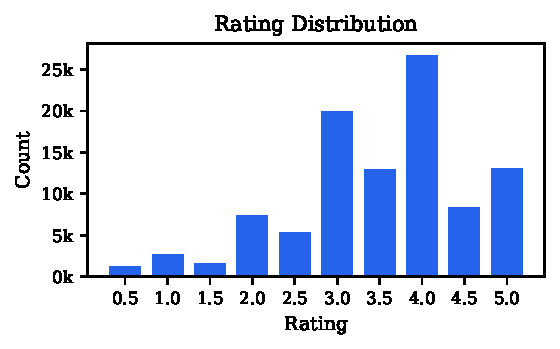
\includegraphics[width=0.85\columnwidth]{rating_dist.pdf}
\caption{Distribution of rating values on MovieLens Latest (counts in thousands on the vertical axis).}
\label{fig:rating_dist}
\end{figure}

\begin{figure}[t]
\centering
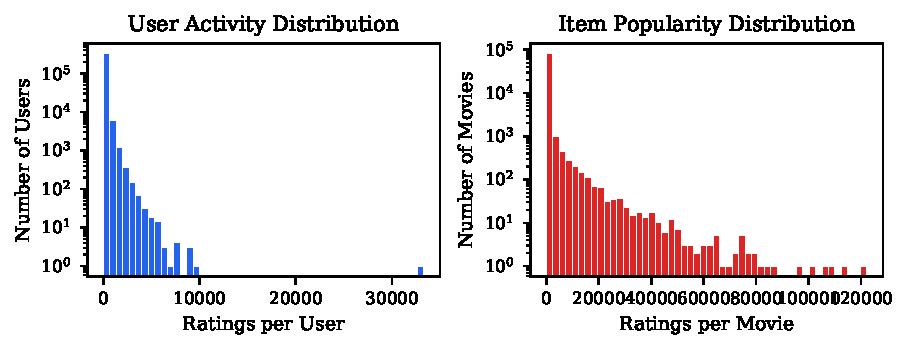
\includegraphics[width=\columnwidth]{user_item_dist.pdf}
\caption{User activity (left) and item popularity (right) on a log-scaled frequency axis, showing heavy-tailed distributions.}
\label{fig:user_item_dist}
\end{figure}

The genre distribution is also imbalanced at the movie-metadata level.
Drama, Comedy, and Thriller dominate the catalog, while niche genres are comparatively rare (Figure~\ref{fig:genre_dist}).

\begin{figure}[t]
\centering
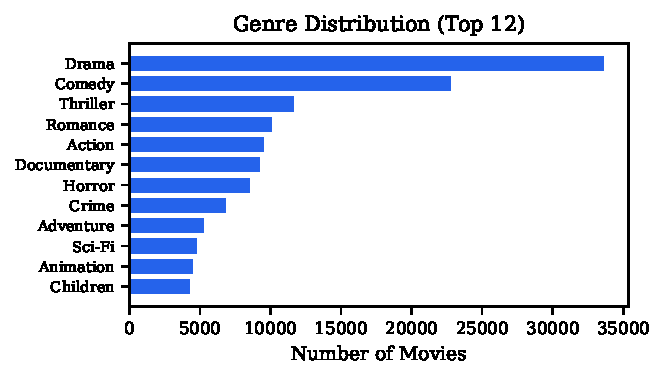
\includegraphics[width=0.9\columnwidth]{genre_dist.pdf}
\caption{Number of movies per genre (top~12).}
\label{fig:genre_dist}
\end{figure}

\paragraph{Data Splitting.}
Following a standard per-user random holdout protocol, for each user we randomly assign 80\% of their ratings to the training set and 20\% to the test set (fixed random seed).
This yields 27{,}065{,}494 training ratings and 6{,}766{,}668 test ratings.
All models share exactly the same split, identified by a deterministic hash for reproducibility.


\section{Experiments}

\subsection{Experimental Setup}

All models are implemented in Python~3.11 with a shared tabular data pipeline.
\textbf{Option~1} (MF-SGD) and \textbf{Option~2} (deep hybrid) were migrated from the earlier NumPy and TensorFlow stack to \textbf{PyTorch}: training uses GPU acceleration when available, Adam-family optimizers with gradient clipping, and large minibatches so that tens of millions of ratings remain tractable in wall-clock time.
\textbf{Option~3} (SVD + Ridge/Lasso) relies on sparse linear algebra and calibrated linear regressors from a standard machine-learning library; \textbf{Option~4} (ALS) is a NumPy-based alternating least-squares loop with validation-based early stopping.

Compared with the earlier small-dataset workflow, we now train and evaluate through one consolidated driver in the repository: MovieLens Latest is the default data source, the per-user 80/20 split is built once and reused for every model so that results are directly comparable, and each training run persists evaluation metrics, serialized parameters, and per-epoch history alongside the corresponding model variant.
Recommended batch sizes for GPU memory and other practical presets are written up separately in the project documentation.

Models are evaluated on the shared test split with two protocols:

\begin{itemize}
\item \textbf{Rating prediction}: MAE and RMSE computed over all 6{,}766{,}668 test ratings.
\item \textbf{Top-10 recommendation}: for each user, the model ranks candidate items by predicted rating and selects the top~10.  Every held-out test item for that user is treated as relevant when computing Precision, Recall, F1, and NDCG (holdout-style evaluation as used in the course setting).
\end{itemize}
To ensure metric reliability across implementations, the evaluation pipeline now includes a consistency guard that checks \texttt{predict\_batch} against scalar \texttt{predict} on a sampled subset and falls back automatically if a mismatch is detected.

\subsection{Hyperparameters}

Table~\ref{tab:hparams} summarizes the key hyperparameters for each model, chosen via preliminary validation-set tuning on MovieLens Latest.

\begin{table}[t]
\centering
\footnotesize
\setlength{\tabcolsep}{3pt}
\begin{tabular}{lcccc}
\toprule
 & \textbf{MF-SGD} & \textbf{Deep} & \textbf{SVD-R/L} & \textbf{ALS} \\
\midrule
$k$ (factors) & 128 & 128 & 128 / 96 & 64 \\
Epochs & 40 & 45 & 1 & 20 \\
Batch size & 65k & 32k & -- & -- \\
Learning rate & 0.0035 & 0.0005 & -- & -- \\
LR decay & $0.995\times$ & plateau & -- & -- \\
Reg.\ $\lambda$ / $\alpha$ & 0.04 & $4{\times}10^{-6}$ $L_2$ & 0.02 / 0.01 & 0.08 \\
Bias reg. & -- & -- & 10.0 & 8.0 \\
Dropout & -- & 0.12 & -- & -- \\
Val.\ split & 0.10 & 0.12 & -- & 0.10 \\
Early stop & pat.\ 4 & best ckpt & -- & pat.\ 4 \\
Loss & MSE & Huber & -- & MSE \\
\bottomrule
\end{tabular}
\caption{Key hyperparameter settings for each model on MovieLens Latest; full command-line presets are in \texttt{docs/TRAINING\_PARAMETERS.md}.}
\label{tab:hparams}
\end{table}


\section{Results and Analysis}

\subsection{Rating Prediction}

Table~\ref{tab:rating_results} reports rating prediction on the 6.77M held-out ratings.
The \textbf{Deep Hybrid} model achieves the best MAE (0.5948), while \textbf{MF-SGD} is now a strong runner-up and attains a marginally lower RMSE (0.8074 vs.\ 0.8075).
\textbf{SVD-Ridge} and \textbf{SVD-Lasso} remain a competitive linear-calibration tier (MAE $\approx$0.667--0.671), and \textbf{ALS} improves compared with earlier presets but still trails the top two models.

\begin{table}[t]
\centering
\small
\begin{tabular}{lcc}
\toprule
\textbf{Model} & \textbf{MAE}$\downarrow$ & \textbf{RMSE}$\downarrow$ \\
\midrule
Deep Hybrid        & \textbf{0.5948} & 0.8075 \\
MF-SGD             & 0.6035 & \textbf{0.8074} \\
SVD-Ridge          & 0.6669 & 0.8671 \\
SVD-Lasso          & 0.6713 & 0.8740 \\
ALS                & 0.6958 & 0.9438 \\
\bottomrule
\end{tabular}
\caption{Rating prediction on MovieLens Latest (per-user 80/20 test split).  Lower is better.}
\label{tab:rating_results}
\end{table}

\begin{figure}[t]
\centering
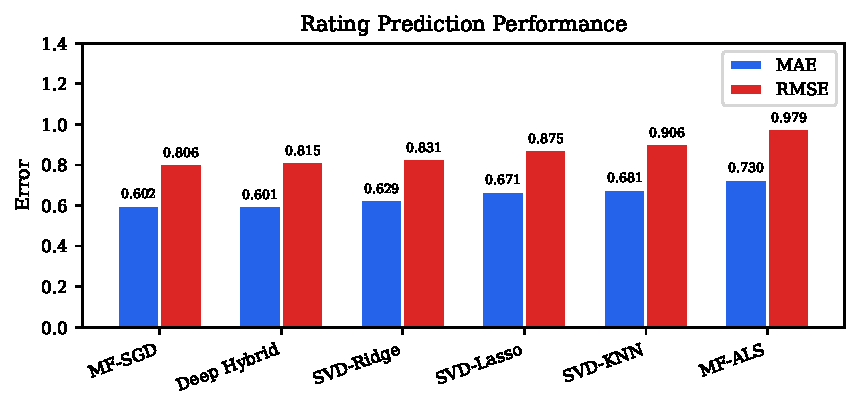
\includegraphics[width=\columnwidth]{model_comparison_rating.pdf}
\caption{Side-by-side MAE and RMSE across all models (MovieLens Latest).}
\label{fig:rating_comparison}
\end{figure}

Training curves illustrate distinct behaviors at scale.
The Deep Hybrid converges smoothly under Huber loss with GPU minibatches (Figure~\ref{fig:deep_curves}).
MF-SGD still reaches its best validation point early and relies on checkpoint restoration (Figure~\ref{fig:mf_curves}), but its tuned configuration now generalizes much better than before.
ALS exhibits the same train--validation divergence pattern under the present $(k{=}64,\lambda{=}0.08)$ configuration, which explains why its ranking metrics remain weak (Figure~\ref{fig:als_curves}).


\subsection{\texorpdfstring{Top-$N$}{Top-N} Recommendation}

\begin{table}[t]
\centering
\footnotesize
\setlength{\tabcolsep}{3pt}
\begin{tabular}{lcccc}
\toprule
\textbf{Model} & \textbf{P@10}$\uparrow$ & \textbf{R@10}$\uparrow$ & \textbf{F1@10}$\uparrow$ & \textbf{NDCG@10}$\uparrow$ \\
\midrule
Deep Hybrid & \textbf{0.0418} & \textbf{0.0368} & \textbf{0.0250} & \textbf{0.0569} \\
MF-SGD      & 0.0355 & 0.0309 & 0.0221 & 0.0502 \\
SVD-Lasso   & 0.0302 & 0.0069 & 0.0093 & 0.0352 \\
SVD-Ridge   & 0.0265 & 0.0054 & 0.0077 & 0.0309 \\
ALS         & 0.0003 & 0.0002 & 0.0001 & 0.0004 \\
\bottomrule
\end{tabular}
\caption{Top-10 recommendation on MovieLens Latest (\texttt{all\_test} relevance).  Higher is better.  Absolute values are small because each user has many held-out test items.}
\label{tab:topn_results}
\end{table}

Table~\ref{tab:topn_results} and Figure~\ref{fig:topn_comparison} summarize ranking metrics.
On this corpus and protocol, the \textbf{Deep Hybrid} model ranks best across Precision, Recall, F1, and NDCG@10.
MF-SGD is now a clear second tier and substantially narrows the gap to Deep Hybrid on all top-10 metrics.
SVD-Lasso slightly edges SVD-Ridge on NDCG, while ALS remains far behind.

The very low ALS top-$N$ scores are consistent with its poor point-wise calibration: when predicted scores poorly separate relevant and irrelevant items, fixed cutoffs at $N{=}10$ collapse precision-oriented metrics.
This is \emph{not} a claim that ALS is inherently unsuitable at scale---only that the present hyperparameters and stopping criterion do not yield competitive scores relative to the deep and SVD-hybrid baselines under identical data conditions.

\begin{figure}[t]
\centering
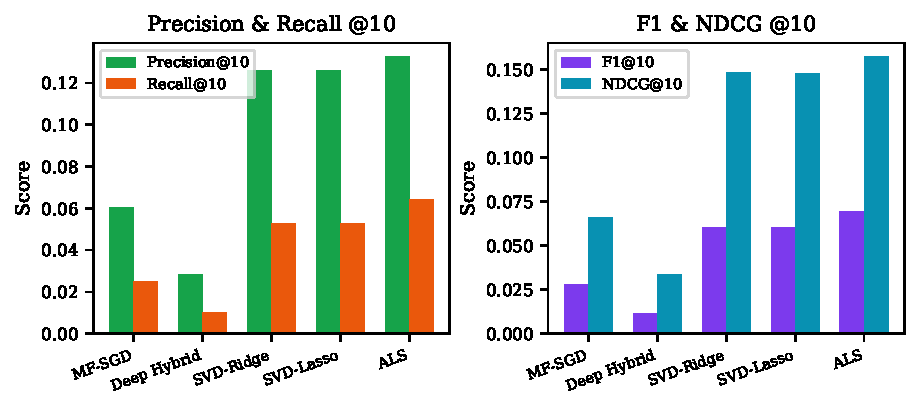
\includegraphics[width=\columnwidth]{model_comparison_topn.pdf}
\caption{Top-10 recommendation metrics across all models (MovieLens Latest).}
\label{fig:topn_comparison}
\end{figure}

To visualize cross-metric trade-offs more directly, we also generate two additional summary plots from the latest \texttt{metrics.json} files.
Figure~\ref{fig:metrics_scatter_radar} (left) shows the MAE--NDCG frontier, where Deep Hybrid and MF-SGD occupy the best region.
Figure~\ref{fig:metrics_scatter_radar} (right) normalizes all five evaluation metrics to compare overall balance across models.

\begin{figure}[t]
\centering
\begin{subfigure}[t]{0.48\columnwidth}
\centering
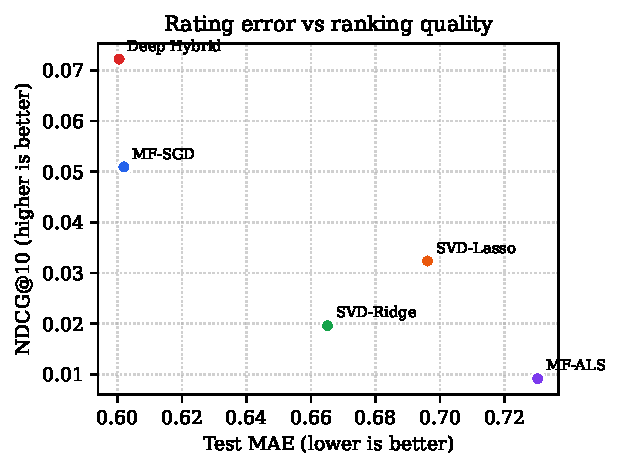
\includegraphics[width=\linewidth]{metrics_scatter_mae_ndcg.pdf}
\caption{MAE vs.\ NDCG@10}
\end{subfigure}
\hfill
\begin{subfigure}[t]{0.48\columnwidth}
\centering
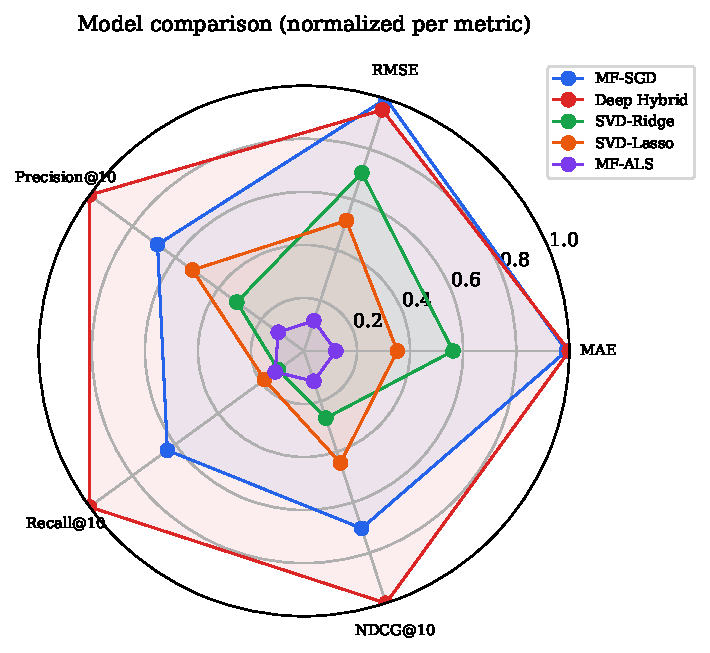
\includegraphics[width=\linewidth]{metrics_radar.pdf}
\caption{Normalized multi-metric radar}
\end{subfigure}
\caption{Additional metrics-summary diagnostics generated by \texttt{scripts/plot\_training\_extras.py}.}
\label{fig:metrics_scatter_radar}
\end{figure}


\subsection{Training Dynamics}

\begin{figure}[t]
\centering
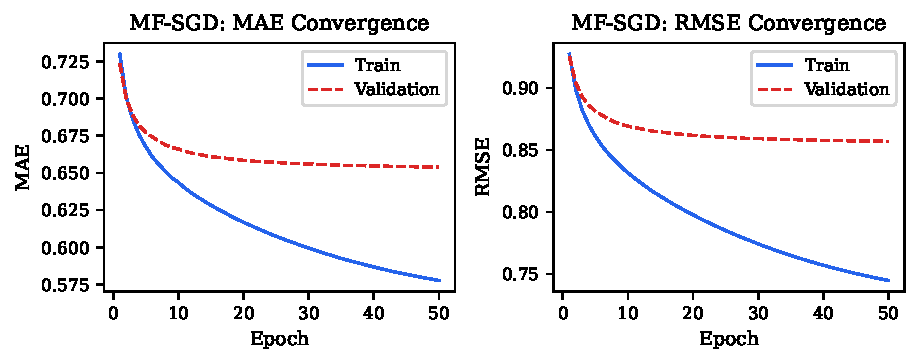
\includegraphics[width=\columnwidth]{training_mf_sgd.pdf}
\caption{MF-SGD on MovieLens Latest: training error decreases while validation MAE/RMSE worsen after the first epochs, motivating early stopping and checkpoint restoration.}
\label{fig:mf_curves}
\end{figure}

\begin{figure}[t]
\centering
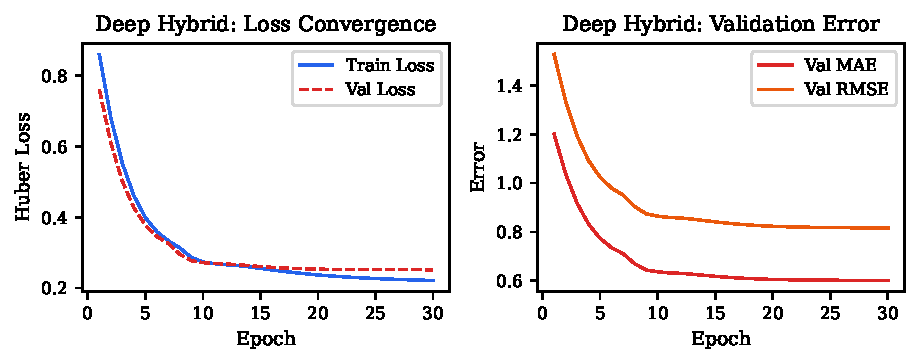
\includegraphics[width=\columnwidth]{training_deep.pdf}
\caption{Deep Hybrid training dynamics under GPU-scale minibatches: Huber loss and validation errors stabilize over 45 epochs with learning-rate reductions on plateau.}
\label{fig:deep_curves}
\end{figure}

\begin{figure}[t]
\centering
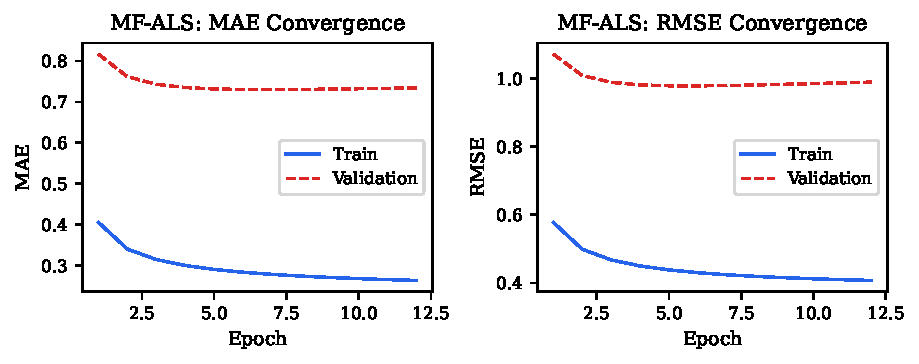
\includegraphics[width=\columnwidth]{training_als.pdf}
\caption{ALS ($k{=}64$, $\lambda{=}0.08$): training error decreases monotonically while validation error plateaus then drifts, indicating a mismatch between the current regularization/rank preset and ranking quality on the full split.}
\label{fig:als_curves}
\end{figure}

The training curves reveal distinct convergence behaviors at web scale:

\paragraph{MF-SGD} (Figure~\ref{fig:mf_curves}) shows rapid initial progress on the training objective, but validation MAE and RMSE reverse direction within the first several epochs.
This pattern is common when aggressively minimizing squared error on massive data without additional ranking-aware objectives.

\paragraph{Deep Hybrid} (Figure~\ref{fig:deep_curves}) benefits from GPU throughput (batch size 32{,}768), Huber robustness, and architectural capacity for content features; validation metrics improve steadily relative to the classical baselines under the same split.

\paragraph{ALS} (Figure~\ref{fig:als_curves}) continues to reduce training error across iterations, yet validation error stops improving early; the restored checkpoint therefore corresponds to a much earlier iterate than the final training state.
In the latest run with this preset, early stopping triggers at epoch 12 and restores the epoch-8 checkpoint.
A dedicated large-scale ALS study (rank sweep, per-block regularization, implicit feedback variants) is left for future work.


\subsection{Feature-Block Ablation}
\label{sec:ablation}

To understand which aspects of the data are most informative for rating prediction beyond collaborative filtering, we previously performed a feature-block ablation using a linear regression model on \textbf{MovieLens-Small} (auxiliary study; Table~\ref{tab:ablation}).
We retain it as qualitative guidance rather than a quantitative claim on MovieLens Latest.

We construct three feature blocks: (1) \textbf{Content} features include genre indicators, genre count, release year, and interaction year; (2) \textbf{Engagement} features include log user activity, log item popularity, log tag count, and log unique tag count; (3) \textbf{Noise} features are two random Gaussian features serving as a control.

\begin{table}[t]
\centering
\small
\begin{tabular}{lccc}
\toprule
\textbf{Feature Block} & $R^2_\text{full}$ & $R^2_\text{w/o block}$ & $\Delta R^2$ \\
\midrule
Full model & 0.1116 & -- & -- \\
\midrule
w/o Content & -- & 0.0582 & 0.0534 \\
w/o Engagement & -- & 0.0815 & 0.0302 \\
w/o Noise (control) & -- & 0.1117 & $-$0.0001 \\
\bottomrule
\end{tabular}
\caption{Auxiliary feature-block ablation (MovieLens-Small, linear probe).  $\Delta R^2$ is the drop in test $R^2$ when a block is removed.}
\label{tab:ablation}
\end{table}

On the small subset, content features account for the largest marginal contribution ($\Delta R^2 = 0.053$), engagement for $\Delta R^2 = 0.030$, and noise is negligible.
These findings still motivate the Deep Hybrid model's incorporation of genre and title features in its item tower, while acknowledging that most variance remains user- and item-specific and is better captured by latent factors.


\subsection{Latent Factor Interpretation}

We interpret latent factors by applying PCA to the item factor matrix $\mathbf{Q}$ learned by MF-SGD and correlating principal components with genre indicators and release year.
On smaller MovieLens slices, such analysis yields semantically coherent axes (e.g., mainstream blockbusters versus critically acclaimed dramas) from collaborative signal alone.
At full scale ($k{=}128$, $|\mathcal{I}|{\approx}8{\times}10^4$ rated items), the same procedure remains a useful qualitative tool, though individual movie exemplars become noisier and less stable across training seeds; we therefore emphasize interpretable \emph{directions} rather than selectively chosen examples.


\section{Discussion}

\paragraph{Rating Accuracy vs.\ Ranking Quality.}
On MovieLens Latest with our evaluation protocol, the Deep Hybrid model leads on \emph{overall} quality: best MAE and best top-10 metrics.
MF-SGD is now close on point-wise error and slightly better on RMSE, but still trails on ranking quality.
This contrasts with our earlier MovieLens-Small study, where stronger regularization on low-rank ALS and SVD hybrids improved NDCG disproportionately.
At tens of millions of ratings, expressive architectures with content channels and GPU-scale optimization can align the two objectives more closely, though MAE/RMSE and ranking metrics still measure different aspects of user utility \cite{rendle2009bpr}.

\paragraph{Classical baselines at scale.}
SVD-Ridge and SVD-Lasso remain attractive: they require only a sparse SVD plus a shallow calibration step, yet achieve MAE below 0.67.
After retuning, MF-SGD is competitive and provides a strong fallback baseline.
ALS remains the weakest model in top-$N$ ranking on this split, which suggests that this explicit-feedback ALS setup still needs deeper rank/regularization redesign.

\paragraph{Depth vs.\ data scale.}
On $\sim$34M interactions, the Deep Hybrid's additional capacity is no longer a pure liability: title CNNs and genre pooling help denoise tail items and improve both RMSE and NDCG relative to the classical runs we report.
The auxiliary linear ablation on MovieLens-Small still suggests that most variance is latent-ID-driven; the deep model's gains likely come from better nonlinear composition of collaborative and content cues rather than from linearly separable metadata alone.

\paragraph{ALS.}
Our ALS configuration ($k{=}64$, stronger $\lambda$) improves rating error compared with our earlier run but still underperforms in ranking quality.
Large-scale ALS typically demands careful rank/regularization search, numerical preconditioning, and sometimes implicit-feedback formulations \cite{hu2008collaborative}; we treat the current numbers as a baseline to improve rather than a fundamental limit of the method.

\paragraph{Demo Application.}
We develop \textit{StreamX}, a full-stack web application consisting of a Django REST API backend and a Next.js frontend.
The backend loads the retrained checkpoints under \texttt{models/artifacts/} and supports switching between them at runtime.
The frontend provides movie browsing, personalized recommendations, TMDB-enriched details, and similar-movie suggestions.



\section{Limitations}

MovieLens Latest is labeled a \emph{development} dataset by GroupLens; snapshots can change, so exact metrics are tied to our July~2023-era checkout.
While we tuned presets documented in the repository, we did not run large-scale automated hyperparameter search for every model; in particular, ALS likely has better operating points than those reported here.
The top-$N$ evaluation uses the \texttt{all\_test} relevance definition (all held-out items are relevant), which yields small absolute Precision/NDCG values when users have many test ratings.
We do not explore temporal dynamics, implicit feedback, or review text beyond titles and genres.
Finally, training deep models assumes GPU availability; CPU-only runs are supported but substantially slower.


\section{Conclusion}

We presented a controlled comparison of four collaborative filtering approaches after migrating from MovieLens-Small to \textbf{MovieLens Latest} and retraining all checkpoints on a shared per-user 80/20 split (27.1M / 6.77M ratings).
Our updated experiments show that (1) the Deep Hybrid model achieves the best overall results (MAE\,=\,0.5948, NDCG@10\,=\,0.0569); (2) tuned MF-SGD becomes a close second and slightly improves RMSE (0.8074 vs.\ 0.8075 for Deep); (3) SVD-Ridge and SVD-Lasso remain solid low-complexity baselines (MAE $\approx$0.667--0.671); and (4) ALS improves in rating error versus earlier presets but remains weak in top-$N$ ranking.

Future work includes dedicated ALS and MF-SGD sweeps at web scale, benchmarking on frozen MovieLens \emph{benchmark} splits for publication-grade comparability, and learning-to-rank objectives that align training with NDCG.

\bibliography{references}

\end{document}
